\section{Analysis and Evaluation}\label{sec-evaluation}
%In this section we report our security analysis and performance evaluation of CAT-SGX.
%In this section, we evaluate our proposal, to see how much the TCB of our system is and each security guarantee that offered by our design, and we show how much additional overhead our CAT-SGX system would cause. 

\subsection{Security Analysis}\label{subsec-securityanalysis}

\noindent\textbf{TCB analysis}. 
The hardware TCB of \textsc{Deflection} includes the TEE-enabled platform, i.e. the SGX hardware. The software TCB includes the components shown in Table~\ref{tb-tcb}. 
The loader we implemented consists of less than 600 lines of code (LoCs) and the verifier includes less than 700 LoCs, also integrating the SGX SDK and part of Capstone libraries. 
The shields of SCONE and Graphene-SGX increase the code size further. Nevertheless, the binary sizes of shielded applications increase to 5 times compared to ours. Currently, Occlum has not integrated the SFI feature in its latest version~\cite{occlum}, thus we can only know the lower bound of its TCB size.
Altogether, our software TCB contains a self-contained enclave binary (1.9 MB) with a shim libc (2.6 MB). By comparison, most solutions are at least an order of magnitude larger as compared to \textsc{Deflection}.

%\wenhao{I think wed better have a table to show all tcb components: categories: SGX SDK/loader/disassembler+rewriter/enforcing policies/}
%According to the threat model~\ref{subsec-threat}, besides the Intel's trusted library - tRTS and the SGX Driver, the software part of the TCB includes the bootstrap enclave software. The SGX hardware, as a TEE-enabled platform, is also part of our TCB on the hardware side. The bootstrap enclave implementation (Section~\ref{subsec:bootstrap-impl}) consists of the loader and the verifier, the wrapped ECall/OCall interfaces, and a simple realization of RA.


\begin{table}[htbp]
\footnotesize
\caption{TCB comparison with other solutions}\label{tb-tcb}
\vspace{-8pt}
\begin{center}
\begin{tabular}{|c|c|c|c|}
\hline
\textbf{Shielding runtimes} & \textbf{Core components} & kLoCs & \textbf{Size(MB)} \\
\hline
 & Eglibc & 892 & \\
Ryoan & NaCl sandbox & 216 & $>$ 19 \\
 & Naclports & 460 & \\
\hline
SCONE & OS Shield and shim libc & 187 & $>$ 16 \\
\hline
 & Glibc & 1200 & \\
Graphene-SGX & LibPAL & 22 & $>$ 58.5 \\
 & Graphene LibOS & 34 & \\
\hline
 & Occlum shim libc & 93 & \\
Occlum & Verifier & N/A & $>$ 8.6 \\
%1.7+2.5+3.1+1.3
 & Occlum LibOS and PAL & 24.5 & \\
\hline
 & Interface and libc & 65  & \\
\textsc{Deflection} & Loader/Verifier & 1.3 & 3.5 \\ 
 & RA/Encryption & 0.2 & \\
\hline
\end{tabular}
\end{center}
%*  Ryoan reports a TCB of multiple modules (including at least a NaCl sandbox), however we do not have the access to the system for comparison.
%* Occlum leverages Rust SGX SDK instead of solely using Intel SGX SDK which is used by other solutions.
\vspace{-10pt}
\end{table}







%%%%----------------------------------------------------------------%%%%
\ignore{

\weijie{comparison}
%\xiaofeng{


\vspace{2pt}\noindent$\bullet$\textit{ Loader and verifier}.
The loader we implemented consists of
%While the main function of dynamic loading we implemented is very small that only consists of 
less than 600 lines of code (LoCs) and the verifier includes less than 700 LoCs, also integrating the SGX SDK and part of Capstone libraries. 
%Yet the whole loader and verifier is supported by the Capstone and an ELF parser so that part of the \verb|libcapstone.a| and the \verb|libelf.a| should also be included.

\vspace{2pt}\noindent$\bullet$\textit{ ECall/OCall stubs for supporting P0}. This was implemented in less than 500 LoCs. 
%Components to process the input/output and its configuration brings in less than 500 lines.

\vspace{2pt}\noindent$\bullet$\textit{ Simple RA protocol implementation}. The implementation  (Section~\ref{subsec:ra-impl}) is done with about about 200 LoCs.

%\vspace{2pt}\noindent$\bullet$\textit{ Dependencies}. Our framework is built upon several existing libraries, which include the SGX SDK libraries, parts of Capstone libraries, and an ELF parser.
\noindent Altogether, our software TCB contains less than 2000 LoCs and some dependencies, which was compiled into a self-contained binary with 1.9 MB in total. By comparison, XXX includes XXX LoCs, XXX in binary in its TCB, based upon our analysis of its code~\cite{shinde2017panoply}. 
%}
%\weijie{openssl}

}







\ignore{
The loader we implemented consists of
%While the main function of dynamic loading we implemented is very small that only consists of 
less than 600 lines of code (LoCs) and the verifier includes less than 700 LoCs, which also integrates SGX SDK and part of Capstone libraries. 
%Yet the whole loader and verifier is supported by the Capstone and an ELF parser so that part of the \verb|libcapstone.a| and the \verb|libelf.a| should also be included.

\vspace{2pt}\noindent$\bullet$\textit{ ECall/OCall stubs for supporting P0}. This was implemented in less than 500 LoCs. 
%Components to process the input/output and its configuration brings in less than 500 lines.

\vspace{2pt}\noindent$\bullet$\textit{ Simple RA protocol realization}. The implementation  (Section~\ref{subsec:ra-impl}) introduces about 200 LoCs.

%\vspace{2pt}\noindent$\bullet$\textit{ Dependencies}. Our framework is built upon several existing libraries, which include the SGX SDK libraries, parts of Capstone libraries, and an ELF parser.
\noindent Altogether, our software TCB contains less than 2000 LoCs and some dependencies, which was compiled into a self-contained binary with 1.9 MB in total.
\weijie{openssl}
}

\vspace{3pt}\noindent\textbf{Policy analysis}. 
Here we show how the policies on the untrusted code, once enforced, prevent information leaks from the enclaves. In addition to side channels, there are two possible ways for a data operation to go across the enclave boundaries:
%Path to the outside of an Enclave includes only two aspects - 
bridge functions~\cite{van2019tale} and memory write.

\vspace{2pt}\noindent$\bullet$\textit{ Bridge functions}. 
With the enforcement of P0, the loaded code can only invoke our OCall stubs, which prevents the leak of plaintext data through encryption and controls the amount of information that can be sent out.
%(to the code provider in CDaaS).
%. With the ECall/OCalls which are to process input/output messages will not reach the plain-text data directly.

\vspace{2pt}\noindent$\bullet$\textit{ Memory write operations}. All memory writes, both direct memory store and indirect register spill, are detected and blocked. Additionally, software DEP is deployed so the code cannot change itself.  Also the control-flow integrity (CFI) policy, P5, prevents the attacker from bypassing the checker with carefully constructed gadgets by limiting the control flow to only legitimate target addresses. 
%since CFI policies are enforced.

As such, possible ways of information leak to the outside of the enclave are controlled. As proved by previous works~\cite{sinha2015moat,sinha2016design} the above-mentioned policies (P1-P5) guarantee the property of confidentiality. Furthermore the policy (P5) of \textit{protecting return addresses and indirect control flow transfer, together with preventing writes to outside} has been proved to be adequate to construct the confinement~\cite{schuster2015vc3,sinha2016design}. So, enforcement of the whole set of policies from P0 to P5 is sound and complete in preventing explicit information leaks. 
In the meantime, our current design is limited in side-channel protection. We can mitigate the threats of page-fault based attacks and exploits on L1/L2 cache once Hyper-threading is turned off or HyperRace~\cite{chen2018racing} is incorporated (P6). However, defeating the attacks without triggering interrupts, such as inference through LLC is left for future research.  



%\subsection{Use Cases and Leakage Control}\label{subsec:usecases}
%\weijie{we can close most covert channels via P0}


%Our security analysis (Section~\ref{subsec-securityanalysis}) has shown that CAT-SGX can prevent explicit data leak. Here we further demonstrates that even though CAT-SGX cannot eliminate the covert channel threat, it provides a level of privacy protection that existing shielding runtimes cannot achieve. 

%for page limit
\ignore{
\vspace{2pt}\noindent\textbf{Covert-channel mitigation}. Since the data owner is the recipient of an enclave's output, all a malicious enclave program can do is to signal to the untrusted OS the content of the data through covert channels, e.g., through system call interfaces. To address this type of covert channel leak, we can control the enclave program's input and output behaviors. One approach is to restrict it, making a single ECall for data input and a single OCall for result output. Consider that the time granularity of the attacker's observation is $R$ (e.g., second), and the time interval of the input/output pair is $T$. The amount of the information (in bit) the attacker can get out to the OS becomes $L_{et} = \log_2 {(T/R)}$. What our approach can do is to modulate this interval, e.g., fixing it to a maximum duration or rounding it to a multiple of a time unit like a minute, so as to control the leak.  Also, all outputs from the enclave are padded to the same size, to avoid the leak through packet length.
}

%As mentioned earlier, covert channels can also be built through SGX hardware, such as cache, memory management, etc. CAT-SGX mitigates such threats through enforcement of P6. 
With such protection, still our design cannot eliminate all covert channels, which is known to be hard. However, it is important to note that other SGX runtimes, including SCONE, Graphene-SGX, Occlum, provide no such protection at all. An exception is Ryoan, which pads its enclave output to the same size, as we do. However, it does not handle the leak from the hardware-based channels.

%Besides, side channel induced by shared hardware can also contribute to some data leak, yet novel transient side channel attacks may leak a few bits~\cite{canella2019systematic}, which can be mitigated via P6 or more alternative policies.





%\noindent\textbf{HTTPS server}. We further looked into another realistic and more complicated case.


%\weijie{Image processing. Image classification as a service is an emerging area.we consideredthat  a  batch  of  one  user’s  data  was  sent  for  processing,  withvarious batch sizes. }




\subsection{Performance Evaluation}\label{subsec-experiments}


\revise{
Here we discuss  performance overhead of different level protections \textsc{Deflection} can provide. These settings include just explicit memory write check (P1), both explicit memory write check and implicit stack write check (P1+P2), all memory write and indirect branch check (P1-P5), and together with side channel mitigation (P1-P6).}
%\weijie{need to modify all P7 to something else}
%\weijie{less narrative, more analysis}

%We evaluated the performance of our implementation on various settings. 


%now focus on the overhead evaluation. The benchmarks include various workloads. We quantify the time and space costs of our prototype by enforcing the execution of the described policies.
%\wenhao{talk about the goal for evaluation}


\noindent\textbf{Testbed setup}. 
%As same as the implementation, our evaluation was also completed on Linux/x86. 
In our research, we evaluated the performance of our prototype and tested its code generation and code execution. All experiments were conducted on Ubuntu 18.04 (Linux kernel version 4.4) with SGX SDK 2.5 installed on Intel Xeon CPU E3-1280 with 64GB memory.
%The maximum heap size and maximum stack size set by all enclaves during testing are 0x2000000 and 0x1800000, respectively. The version of SGX driver we use is 2.
%However, Intel has not shipped SGXv2 CPUs widely. So we evaluate the \textsc{Deflection} model on SGXv1 to show its compatibility.
Also we utilized  GCC 5.4 to build the bootstrap enclave and the SGX application, and the parameters `-fPIC', `-fno-asynchronous-unwind-tables', `-fno-addrsig', and `-mstackrealign' to generate x86 binaries. 

%for page limit
\ignore{
\begin{table}[htbp]
\footnotesize
\caption{Additional code size and execution time}\label{tb-simple-perf}
\vspace{-5pt}
\begin{center}
%\begin{tabular}{|c|c|c|c|c|c|c|c|c|c|}
\begin{tabular}{|c|cc|cc|}
\hline
%\textbf{Application Name} & \textbf{Size} & \textbf{Size (P1\textasciitilde P5)} & \textbf{Size (P1\textasciitilde P5+P6)} & \textbf{Size (P1\textasciitilde P5+P6-SSA)} & \textbf{Time} & \textbf{Time (P1\textasciitilde P5)} & \textbf{Time (P1\textasciitilde P5+P6)} & \textbf{Time (P1\textasciitilde P5+P6-SSA)}\\
%\textbf{Application Name} & \textbf{Size} & \textbf{Size (P1\textasciitilde P5)} & \textbf{Size (P1\textasciitilde P6)} & \textbf{Execution Time} & \textbf{Execution Time (P1\textasciitilde P5)} & \textbf{Execution Time (P1\textasciitilde P6)}\\
\textbf{Application} & \textbf{Size(P1-P5)} & \textbf{(P1-P6)} & \textbf{Time(P1-P5)} & \textbf{(P1-P6)}\\
%\hline
%bm\_hello.c & 3.6K & 1.218s \\
\hline
clock & +3.83\% & +4.31\% & +14.6\% & +15.8\% \\
\hline
malloc\_and\_magic & +4.41\% & +5.29\% & +14.4\%  & +22.0\% \\
\hline
malloc\_memalign & +4.80\% & +5.68\% & +14.8\% & +22.6\% \\
\hline
malloc\_and\_sort & +6.73\% & +8.17\% & +16.0\% & +27.6\% \\
\hline
memcpy & +68.1\% & +134\% & +2.97\% & +15.3\% \\
\hline
memchr & +59.6\% & +116\% & +3.39\% & +15.0\% \\
\hline
sprintf & +5.71\% & +8.57\% & +6.65\% & +18.2\% \\
\hline
sort\_and\_binsearch & +10.1\% & +14.6\% & +6.48\% & +18.3\%\\
\hline
Average & +\% & +\% & +\% & +\%\\
\hline 
\end{tabular}
\end{center}
\vspace{-8pt}
\end{table}



\vspace{3pt}\noindent\textbf{Performance on simple applications}. We used the applications provided by the SGX-Shield project~\cite{seo2017sgx} as a micro-benchmark. In our experiment, we ran each test case for 10 times, measured the resource consumption in each case and reported the median value. Specifically, we first set the baseline as the performance of an uninstrumented program running through a pure loader (a loader that only does the dynamic loading but no policy-compliance checking). Then we compared the baseline with the performance of instrumented programs to measure the overheads. Also the compilation time of each micro-benchmark varies from several seconds to tens of seconds, which is negligible compared with conventional PCC methods (2-5$\times$)~\cite{necula2001oracle}.
%measured the runtime overhead and  the baseline being an uninstrumented program running in a pure loader (a loader that only does the dynamic loading but no policy-compliance checking). Then we instrumented those programs and measure the execution time. The compilation time of each micro-benchmark varies from several seconds to tens of seconds, which is negligible compared with conventional PCC methods (2\textasciitilde 5$\times$)~\cite{necula2001oracle}.
%\wenhao{show how long PCC takes}
%on simple application bench
%geometry mean of performance overhead of P1~P5: 1.098
%geometry mean of performance overhead of P1~P6: 1.193
%geometry mean of storage overhead of P1~P5: 1.181
%geometry mean of storage overhead of P1~P6: 1.295

Table~\ref{tb-simple-perf} illustrates overheads of our approach. 
From the table, we can see that the size of instrumented binaries (a.k.a. the ``code + proof'') is 18.1\% larger than the original code and their executions were delayed by 9.8\% on average
when only P1-P5 are enforced. The overhead becomes 30\% in memory and 19\% in time when all policies, including P6, are enforced. Note that this batch of benchmarks are mostly a `first-simple-processing-then-syscall' program. At the worst case - `malloc\_and\_sort', \textsc{Deflection} showed 27.6\% overhead in execution time. 
}

\begin{table}[htbp]
\footnotesize
\caption{Performance overhead on nBench}\label{tb-nben-perf}
\vspace{-5pt}
\begin{center}
\begin{tabular}{|c|c|c|c|c|}
\hline
\textbf{Program Name} & \textbf{P1} & \textbf{P1+P2} & \textbf{P1-P5} & \textbf{P1-P6}\\
\hline
NUMERIC SORT  & +5.18\% & +6.05\% & +6.79\% & +12.0\% \\
\hline
STRING SORT  & +8.05\% & +10.2\% & +12.4\%  & +18.4\% \\
\hline
BITFIELD  & +6.11\% & +11.3\% & +15.5\% & +17.9\% \\
\hline
FP EMULATION  & +0.20\% & +0.27\% & +0.33\% & +5.36\% \\
\hline
FOURIER & +2.48\% & +2.72\% & +2.89\% & +7.45\% \\
\hline
ASSIGNMENT & +6.73\% & +15.6\% & +25.0\% & +39.8\% \\
\hline
IDEA & +2.34\% & +2.66\% & +3.13\% & +12.1\% \\
\hline
HUFFMAN & +15.5\% & +16.6\% & +18.1\% & +21.3\% \\
\hline
NEURAL NET  & +13.8\% & +19.4\% & +20.2\% & +23.1\% \\
\hline
LU DECOMPOSITION  & +4.30\% & +7.03\% & +9.67\% & +22.6\% \\
\hline
\end{tabular}
\end{center}
\vspace{-10pt}
\end{table}

\vspace{3pt}\noindent\textbf{Performance on nBench}. We instrumented all applications in the SGX-nBench~\cite{sgxnbench}, and ran each testcase of the nBench suites under a few settings, each for 10 times. 
%These three versions of Code Generators were also used in later performance evaluation.
Table~\ref{tb-nben-perf} shows the average execution time under different settings.
Without side channel mitigation (P1-P5), our prototype introduces an 0.3\% to 25\% overhead (on FP-emulation). %The Assignment algorithm - a well-known task allocation algorithm - has the largest overhead, with 6.7\% for just enforcing P1. 
Apparently, the store instruction instrumentation alone (P1) does not cause a large performance overhead, with largest being 6.7\%. Also, when P1 and P2 are applied together, the overhead just becomes slightly higher than P1 is enforced alone. %For instance, on Numeric Sort, the increasing overhead is about 6.1\% more than the baseline, and 0.8\% more than the one with just explicit memory write check. 
Besides, almost all benchmarks in nBench perform well under the CFI check P5 (less than 3\%) except for the benchmarks Bitfield (about 4\%) and the Assignment (about 10\% due to its frequent memory access pattern).

\vspace{3pt}\noindent\textbf{Performance on real-world applications}.  We further evaluated our prototype on various real-world applications, including personal health data analysis, personal financial data analysis, and Web servers. 
%Firstly, we chose sequence generation and alignment algorithms as representative benchmarks, which are widely used in genome data analysis. 
We implemented those macro-benchmarks and measured the differences between their baseline performance (without instrumentation) in enclave and the performance of our prototype.


\vspace{2pt}\noindent$\bullet$\textit{ Sensitive genome data analysis}. We implemented the Needleman–Wunsch algorithm~\cite{needleman1970general} that aligns two human genomic sequences in the FASTA format~\cite{fasta-format} taken from the 1000 Genomes project~\cite{1000genomes}. The algorithm uses dynamic programming to compute recursively a two dimensional matrix of similarity scores between subsequences; as a result, it takes $N^2$ memory space where $N$ is the length of the two input sequences. 
We measured the sequence alignment program execution time under the aforementioned settings. Figure~\ref{fg-nw-perf} shows the performance of the sequence alignment algorithm with different input lengths (x-axis). The overall overhead (including all kinds of instrumentations) is no more than 20\% (with the P1 alone no more than 10\%), when input size is small (less than 200 Bytes). When input size is greater than 500 Bytes, the overhead of P1+P2 is about 19.7\%  while P1-P5 spends 22.2\% more time than the baseline.

\begin{figure*}[htbp]
\begin{center}
\begin{minipage}[t]{0.33\linewidth}
    \centering
    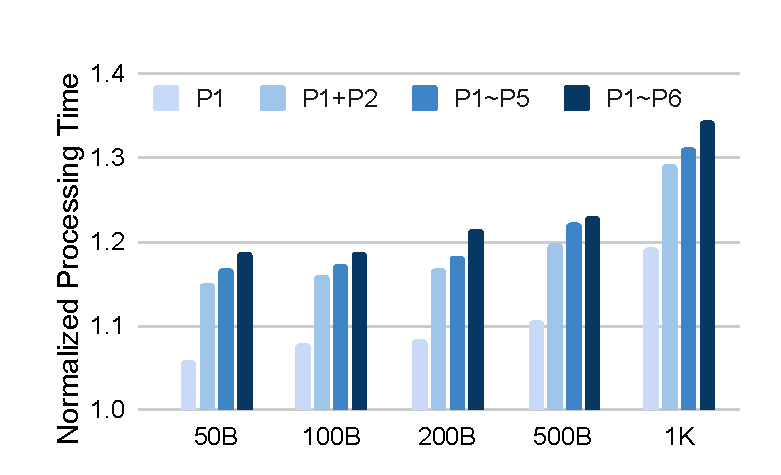
\includegraphics[scale=0.46]{figures/fg-nw-perf.pdf}
    \caption{Sequence alignment}\label{fg-nw-perf}
\end{minipage}
\begin{minipage}[t]{0.33\linewidth}
    \centering
    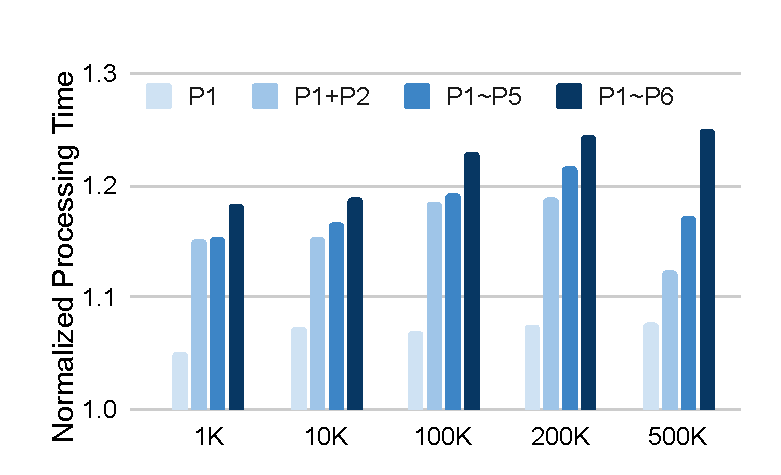
\includegraphics[scale=0.46]{figures/fg-fasta-perf.pdf}
    \caption{Sequence generation}\label{fg-fasta-perf}
\end{minipage}
\begin{minipage}[t]{0.32\linewidth}
    \centering
    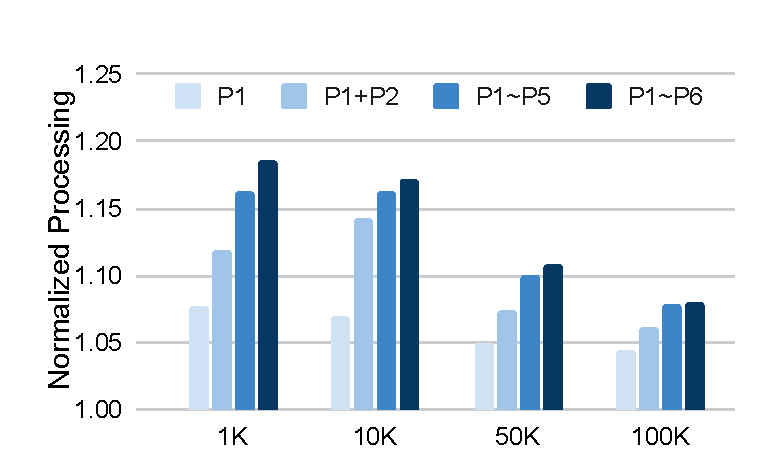
\includegraphics[scale=0.46]{figures/fg-credit-score.pdf}
    \caption{Credit scoring}\label{fg-credit-score}
\end{minipage}
\end{center}
\vspace{-12pt}
\end{figure*}
%\begin{figure}[htbp]
\centerline{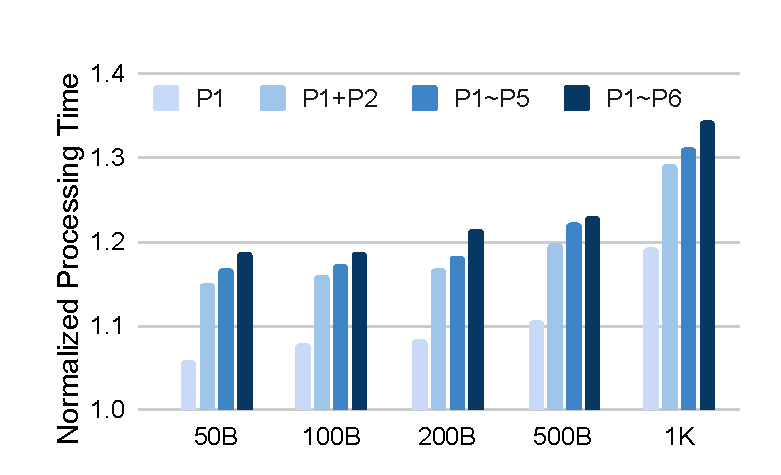
\includegraphics[scale=0.48]{figures/fg-nw-perf.pdf}}
\caption{Performance on sequence alignment}\label{fg-nw-perf}
\end{figure}
%\begin{figure}[htbp]
\centerline{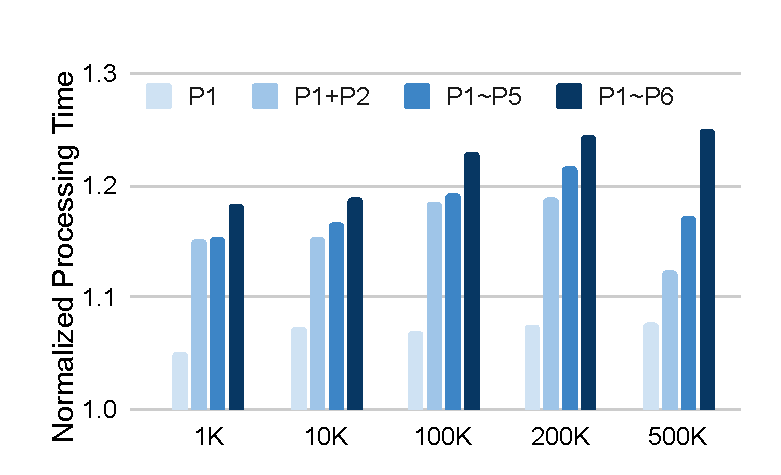
\includegraphics[scale=0.48]{figures/fg-fasta-perf.pdf}}
\caption{Performance on sequence generation}\label{fg-fasta-perf}
\end{figure}
%\begin{figure}[htbp]
\centerline{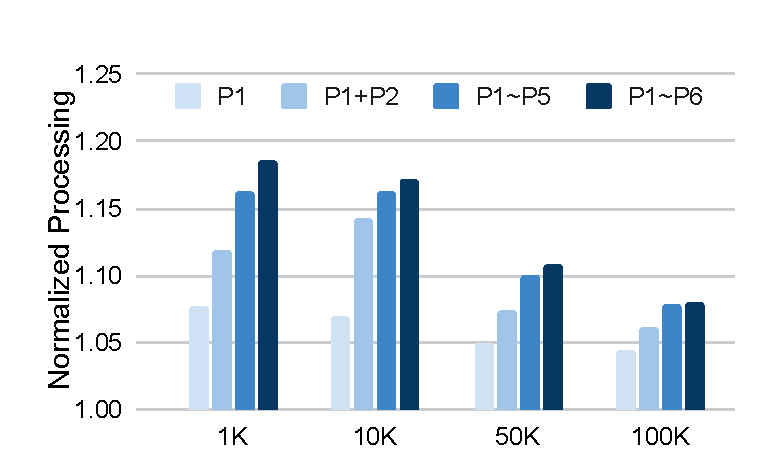
\includegraphics[scale=0.48]{figures/fg-credit-score.pdf}}
\caption{Performance on credit scoring}\label{fg-credit-score}
\end{figure}

For sequence generation, Figure~\ref{fg-fasta-perf} shows the performance when the output size (x-axis) varies from 1K to 500K nucleotides. Enforcing P1 alone results in 5.1\% and 6.9\% overheads when 1K and 100K are set as the output lengths. When the output size is 200K, our prototype yields less than 20\% overhead. Even when the side channel mitigation is applied, the overhead becomes just 25\%. With the increase of processing data size, the overhead of the system also escalates; however, the overall performance remains acceptable.


\vspace{2pt}\noindent$\bullet$\textit{ Personal credit score analysis}. In our study, we implemented a BP neural network-based credit scoring algorithm~\cite{jensen1992using} that calculates user's credit scores. The model was trained on 10000 records and then used to make prediction (i.e., output a confidence probability) on different test cases.
As shown in Figure~\ref{fg-credit-score}, on 1000 and 10000 records, enforcement of P1-P5 would yields around 15\% overhead. 
%Only P1+P2 takes more than 12\% herein. 
While processing more than 50000 records, the overhead of the full check does not exceed 20\%.  The overhead of P1-P6 does not exceed 10\% when processing 100K records.

\begin{figure}[htbp]
\centerline{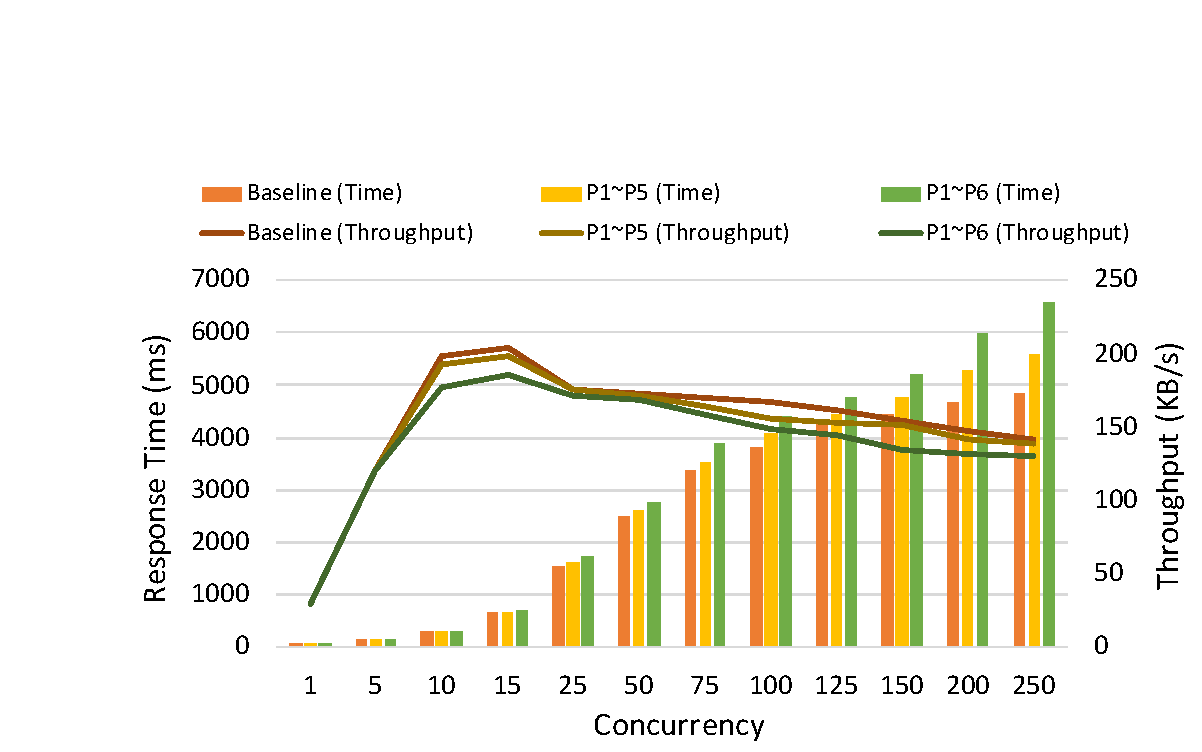
\includegraphics[scale=0.48]{figures/fg-https-server.pdf}}
\vspace{-2pt}
\caption{Performance on HTTPS server}\label{fg-https-all}
\vspace{-15pt}
\end{figure}
%\begin{figure}[htbp]
\centerline{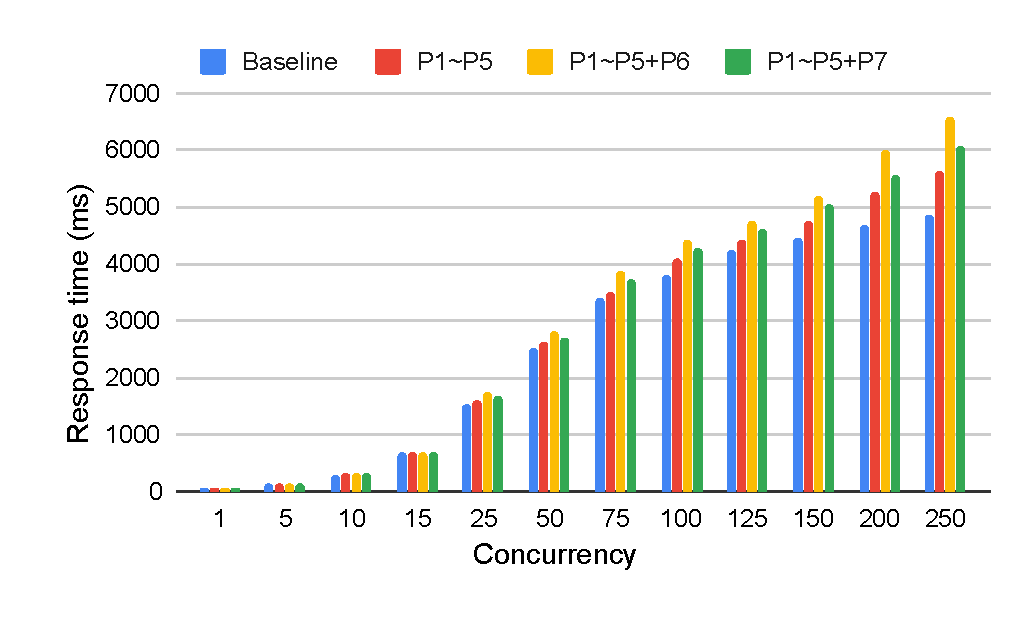
\includegraphics[scale=0.5]{figures/fg-https-rs.pdf}}
\caption{Performance on HTTPS Server (Response Time)}\label{fg-https-rs}
\end{figure}

\vspace{2pt}\noindent$\bullet$\textit{ HTTPS server}. We built an HTTPS server in enclave using the mbed TLS library~\cite{mbedtls}. 
%Our protection only allows two system calls (\texttt{send/recv}) to be executed via the OCall stubs for client/server communication. 
A client executes a stress test tool - Siege~\cite{siege} - on another host in an isolated LAN. Siege was configured to send continuous HTTPS requests (with no delay between two consecutive ones) to the web server for 10 minutes. We measured its performance in the presence of different concurrent connections to understand how our instrumented HTTPS server implementation would perform. 
%One concurrent request is deployed for measuring the response time. 

%\begin{figure}[htbp]
\centerline{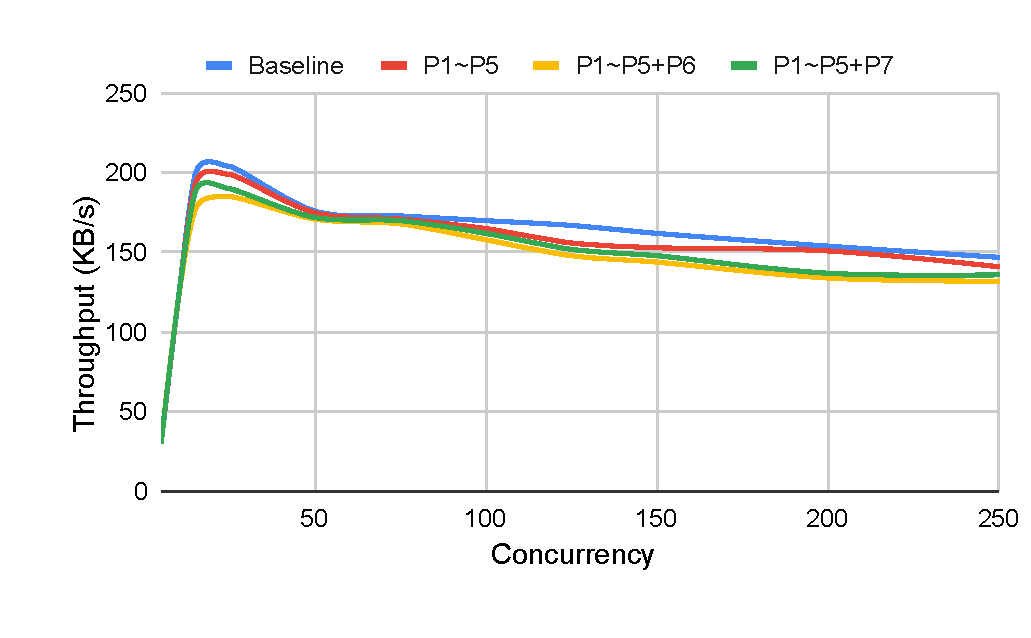
\includegraphics[scale=0.5]{figures/fg-https-tp.pdf}}
\caption{Performance on HTTPS Server (Throughput)}\label{fg-https-tp}
\end{figure}

Figure~\ref{fg-https-all} shows the response times and throughput when all policies are applied to the HTTPS server benchmark. When the concurrent connections are less than 75, the instrumented HTTPS server has similar performance of the in-enclave https server without instrumentation. When the concurrency increases to 100, the performance goes down to some extent. 
While after the concurrency increases to 150, the response time of instrumented server goes up significantly. On average, enforcing P1-P6 results in 14.1\% overhead in the response time. As for throughput, when the number of the concurrent connections is between 75 and 200, the overhead is less than 10\%. 
%the baseline always achieveshigher throughput, though just less than 10\% higher. 
These experiments on realistic workloads show that all policies, including side-channel mitigation, can be enforced at only reasonable cost. 

%proper policies on side channel mitigations can be enforced with only reasonable overhead.

\vspace{3pt}\noindent\textbf{Performance comparison on HTTPS server}.
Here we compare the performance overheads induced by existing shielding runtimes with our solution. Since Occlum has not integrated the SFI feature in its latest version~\cite{occlum} and Graphene-SGX does not support our security policies, we cannot get their performance details to compare against ours when policy-enforcing instrumentations are added. In our study, we ran an HTTPS server within those runtimes. As expected, their performance is affected by the workload, sizes of files requested from the server. As shown in Figure~\ref{fg-comparison}, unprotected Graphene-SGX has the best transfer rate with relatively small files. However, with the size growing, \textsc{Deflection} outperforms both runtimes (77\% of running the server on the native Linux), even when our approach implements security policies (P0-P5) while these runtimes do not. 


%Here we compare the performance overhead induced by existing shielding runtimes with our solution.  Since Occlum has not integrated the SFI feature in its latest version~\cite{occlum}, therefore we do not have the performance details on how it performs compared to ours when certain instrumentations were added. Compared with the HTTPS server on native Linux, shielding runtimes have performance discrepancies when requesting different sizes of files. When processing files less than 50MB, Graphene-SGX has the best transfer rate. However, it drops drastically with the file size increasing. Occlum's performance (1 thread, without SFI) also suffers from processing files whose size is larger than 70MB, while our solutions (both with and without policy enforcement) maintain a relatively high level of normalized transfer rate (greater than 77\%).


\begin{figure}[htbp]
\centerline{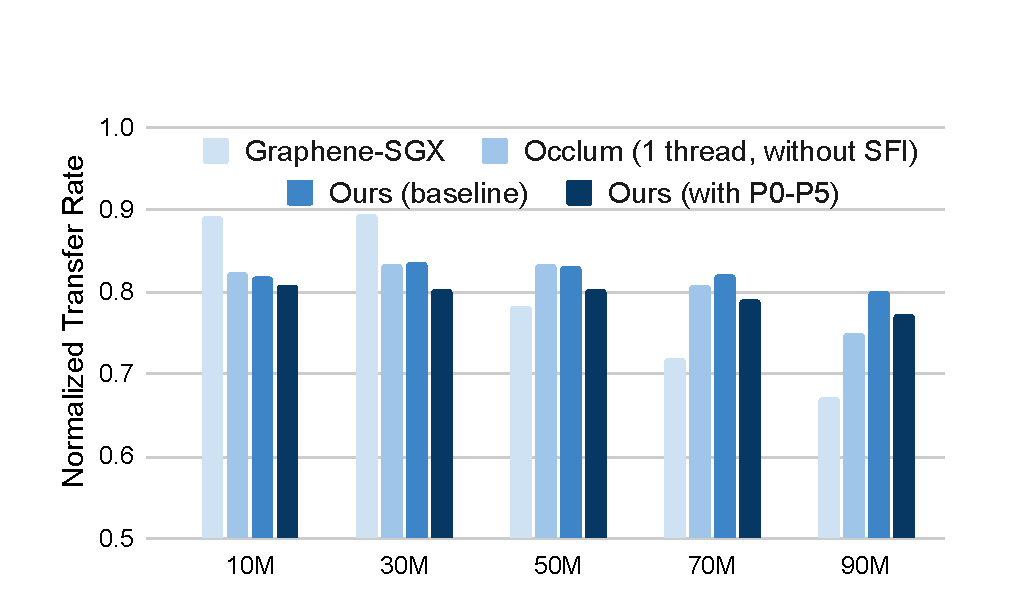
\includegraphics[scale=0.42]{figures/fg-comparison.pdf}}
\vspace{-2pt}
\caption{Performance comparison}\label{fg-comparison}
\vspace{-15pt}
\end{figure}
%\weijie{more distinguishable colors}

\ignore{
Currently, Occlum has not integrated the SFI feature in its latest version~\cite{occlum}, therefore we do not have the performance details on how it performs compared to ours when certain instrumentations were added. Compared with the HTTPS server on native Linux, Graphene-SGX, Occlum, and Ours all fluctuate between from 80\% to 90\%.
The performance of Occlum without SFI and the performance of the baseline CAT prototype (without ) are neck and neck, while Graphene-SGX has the best transfer rate since it does not provide memory access/CFI protection like ours (in Figure~\ref{fg-comparison}). Nevertheless, Graphene-SGX has to create a new enclave for each new process, which is very time consuming~\cite{shen2020occlum}.
The concurrent number ($<= 256$) has slight affect on the network throughput.
}